This chapter explains about the major tasks implemented in the thesis, new contributions made to the PUF Toolkit. The first part of the chapter briefly explains about the current PUF toolkit implementation, without delving much into the details. The second and more major part talks about the new modifications that were done to the toolkit in the form of BCH fuzzy extractor encoder and decoder integration, which were previously not a part of the main toolkit and presented as seperate executables
with seperate menu items. We then go on to explain the Golay code implementation both the decoder and encoder, and explain their integration in the toolkit as a distinct menu item. Then the other modifications like the addition of \emph{'offsets from begining and end', error codes} and other intricate code developement changes are presented together as one section.\\

TODO: write about hamming distance and jaccardi's index

The final two sections deal with cognicrypt details and the Java Native Interface (JNI), they first touch upon the basics of JNI
wrapper and the functioning of JNI with shared libraries packaged as JAR files that are accesible to Java compiler as external library. Finally, we describe the clafer model of the cognicrypt and how it assists users and Java developers, without any previous knowledge about cryptography, to select a strong PUF based secure key evaluation algorithm based on the questions asked by the cognicrypt. In the end of this last section we also talk about the xsl model of the cognicrypt that builds on
the clafer model to generate a boilerplate java code to help the Java developer by presenting him/her with a sample usecase of the Java code implementation showing a usage of the PUF evaluation algorithms that is robust and flawless.\\

For the implementation, the ISO standardize programming language C++ was chosen. This selection was made based on the efficient and general purpose features provided by C++. Apart from the object oriented and generic programming features, C++ has a high abstraction level and the compilation and code development can be done on diverse systems. The implementations are dissociated from a specific hardware to support a wide range of systems and applications. This makes the toolkit easier
to extned and conform to a particular hardware for next iterations. The JNI framework support native calls and the wrapper is written in Java, for clafer model we use Java script and json files along with the .cfr clafer extension modelling language(refer to github page [ ] for details) and xsl model to generate sample Java boilerplate code is written in xsl.\\

\section{PUF Toolkit} 
The current implementation of the PUF toolkit was done and presented in the thesis [sebastian Master Thesis]. The main aim of the toolkit is to evaluate various PUF repsonse based on well established metrics and thereby helping researchers and designers to gain useful insights into the properties and behaviour of PUF responses. The toolkit implements the following list of metrics: \pagebreak

\begin{itemize}
	\item (Shannon) Entropy
	\item Hamming Weight
	\item Intra-Hamming Distance
	\item Inter-Hamming Distance
	\item Min-entropy
	\item Median and average
\end{itemize}

These metrics are well explained in the Master thesis Sebastian [ ], so we take the liberty to not go into the detail of explaining each metric here again. It must also be noted that there are other metrics and definitions that use identical concepts and/or apply the metrics in a different way to generalize the coorelation between different PUF instances and their reponses. More exhaustive and comprehensive information related to these metrics and definitions for PUFs can be found in [seb 37, 53, 26, 5].\\

Apart from the above mentioned metrics implementation the PUF based secure key storage is implemented already, using BCH encoder and Decoder in two seperate executables. The structure and the User design used in these two executables is similar to the PUF toolkit and to avoid confusion we shall refer to them as \emph{PUF-BCH encoder} and \emph{PUF-BCH decoder}.\\

\subsection{User Design}

The notion behind the console user interface design by inspired from Nielsen and Molich's nine user interface design guidelines [seb 45]. These guidelines and their resulting effects are shown the table \ref{tab:guidline_design} below:

\begin{table}[!ht]
\begin{center}
\begin{tabular}{cll}
\toprule
\multicolumn{1}{c}{\textbf{No.}} &\multicolumn{1}{c}{\textbf{Guideline}} & \multicolumn{1}{c}{\textbf{Effect}}\\
\midrule
\hline
1 & Simple and natural dialogue & Clear and logical dialogue structure\\

2 & Speak the user’s language & Clear instructions\\

3 & Minimize the user’s memory load & Clean design, brief help and guide texts\\

4 & Be consistent & Consistent design in all menus\\

5 & Provide feedback & Provide feedback and status\\

6 & Provide clearly marked exits & Provide ``back’’ and ``exit’’ in each menu\\

7 & Provide shortcuts & Inputs by abbreviations \\

8 & Good error messages & Provide useful error messages\\

9 & Prevent errors & Handle wrong inputs \\
\hline
\addlinespace
\bottomrule
\end{tabular}
\end{center}
\caption{The nine design guidelines according to [seb 45] and the effect on the UI design.}
\label{tab:guidline_design}
\end{table}

The design of the menu and the (sub-) menus is consistent and recurses itself to make the user interface more intuitive and friendly. Each menu option is written in clear and easy to understand instructions and the menu items are precisely structured to help the user navigate the toolkit with ease. The organization of the menu follows a hierarchical design and a ``back'' function is provided for the user to go to the parent menu. A conceptual depiction of the User Interface is shown in Figure
\ref{img:gui_design}. The Graphical User Interface (GUI) is subdivided into four parts, the color markers are related to the illustration in \ref{img:gui_design}:

\begin{itemize}
	\item The first part, marked in yellow, is the \emph{header}. It gives the user general information, like the title of the current (sub-) menu or brief instructions.
	\item The second part of the gui shows the options and functions that the user can choose from the (sub-) menu, the number infront must be input by the user in the last part of the GUI. The conceptual illustration for the part is marked in red and is called as \emph{Menu}.
	\item Below the Menu part there is \emph{settings and results} that are marked in blue. It shows the current configuration and provides the user with essential information that is vital for the actual computation of the main function. It also shows the output after the computation is performed in the result part of this section.
	\item The fourth part of the GUI is for \emph{feedback} and inputs and is marked in green. It presents the user with the actual processing status, or if an error occurred and the type of the error. Also, it contains a user interactive input cursor, a number must be typed in by the user in order to select the options/functions from the second part, Menu of the GUI.
\end{itemize}

\begin{figure}
\centering
\fbox{ 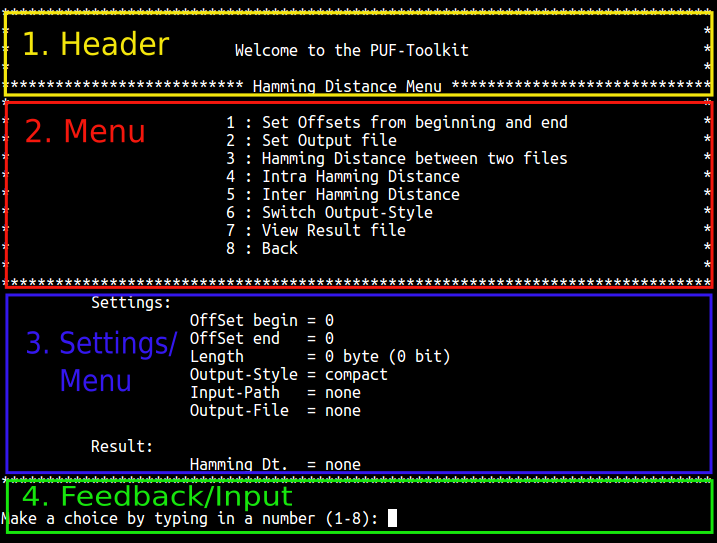
\includegraphics[width=0.9\textwidth]{images/toolkit_gui4.png}}
\caption{Conceptual design of the PUF Toolkit user interface.}
\label{img:gui_design}
\end{figure}

The design of the GUI is kept simple without the use of extended graphic components to keep the toolkit compatible with other operating systems like linux. The UI shows only relevant information depending on the current state of the program and potrays a simple but aesthetic clean design. Error correction and incorrect user input is efficiently handled, all possibile inputs are exhausted and depeding on the false input, meaningful errors information is displayed to the user, that can be used to
recover from the erroneous state. Also for all mandatory inputs a brief guide / help text with examples is shown, the current settings are saved and kept in each (sub-) menu (wherever applicable) to avoid unecessary redudant input.\\

By strictly adhering to the design guidelines throughout the toolkit, an effective and intuitive console
user interface was created. The developed console user interface can thereby decisively support designers
and researchers in the evaluation of PUFs. [seb thesis]
